%
% File semeval2020.tex
%
% Nathan Schneider
%% Based on the style files for COLING-2020 (feiliu@cs.ucf.edu & liang.huang.sh@gmail.com), which were, in turn,
%% Based on the style files for COLING-2018, which were, in turn,
%% Based on the style files for COLING-2016, which were, in turn,
%% Based on the style files for COLING-2014, which were, in turn,
%% Based on the style files for ACL-2014, which were, in turn,
%% Based on the style files for ACL-2013, which were, in turn,
%% Based on the style files for ACL-2012, which were, in turn,
%% based on the style files for ACL-2011, which were, in turn,
%% based on the style files for ACL-2010, which were, in turn,
%% based on the style files for ACL-IJCNLP-2009, which were, in turn,
%% based on the style files for EACL-2009 and IJCNLP-2008...

%% Based on the style files for EACL 2006 by
%%e.agirre@ehu.es or Sergi.Balari@uab.es
%% and that of ACL 08 by Joakim Nivre and Noah Smith

\documentclass[11pt]{article}
\usepackage{geometry}
\usepackage{coling2020}
\usepackage{times}
\usepackage{url}
\usepackage{latexsym}
\usepackage{microtype}
\usepackage{booktabs}
\usepackage{graphicx}
\usepackage{courier}
\usepackage{multirow}
\usepackage{floatrow}
% Table float box with bottom caption, box width adjusted to content
\newfloatcommand{capbtabbox}{table}[][\FBwidth]

\hyphenation{an-aly-sis}
\hyphenation{an-aly-ses}
\hyphenation{Sem-Eval}
%\setlength\titlebox{5cm}
\colingfinalcopy % Uncomment this line for all SemEval submissions

% You can expand the titlebox if you need extra space
% to show all the authors. Please do not make the titlebox
% smaller than 5cm (the original size); we will check this
% in the camera-ready version and ask you to change it back.


\title{T\"uKaPo at SemEval-2020 Task 6: Def(n)tly not BERT:\\
Definition Extraction using pre-BERT Methods in a post-BERT World}

\author{Madeeswaran Kannan\thanks{\quad mkannan@sfs.uni-tuebingen.de} \qquad Haemanth Shanthi Ponnusamy\thanks{\quad haemanth.santhi-ponnusamy@student.uni-tuebingen.de}\\
	Department of Linguistics \\
	University of T\"ubingen, Germany \\}


\date{}

\begin{document}
\setlength{\parindent}{0pt}.

\maketitle
\begin{abstract}
  We describe our system (T\"{u}KaPo) submitted for Task 6: DeftEval, at SemEval 2020.
  We developed and evaluated multiple neural network models based on CNNs and LSTMs to
  perform binary classification of sentences containing definitions. Our final model
  achieved a F1-score of $0.6851$ in subtask 1.
\end{abstract}

\renewcommand*{\arraystretch}{1.0}

\blfootnote{
    \hspace{-0.65cm}  % space normally used by the marker
    This work is licensed under a Creative Commons
    Attribution 4.0 International License.
    License details:
    \url{http://creativecommons.org/licenses/by/4.0/}.
}

\section{Introduction}
By most accounts, the first reliable English dictionary was written by Samuel Johnson\footnote{\url{https://en.wikipedia.org/wiki/A_Dictionary_of_the_English_Language}} and published on 15 April, 1755. It was 18 inches tall, 20 inches wide when opened, and
contained 42,773 entries. It took Dr. Johnson 7 years to complete, and yet it was missing the word \emph{contrafibularity}, amongst others\footnote{\emph{Aardvark} was another.}. In the 265 years that have passed since, the world has evolved at a blisteringly fast
pace with technology integrating itself ever more closely with our lives. However, the compilation and maintenance of dictionaries and
lexicons - one of the most important and authoritative sources of meaning - continues to be the exclusive field of domain experts
and lexicographers. Nevertheless, with the recent advances in natural language processing, this area - like many others that deal
with human language - has seen a growing interest in automating the development of such resources.\\

Definition extraction is defined as the automatic identification of definitional knowledge in text, modeled as a binary
classification problem between definitional and non-definitional text. In the early days of definition extraction,
rule-based approaches leveraging linguistic features showed promise. \newcite{westerhout2009definition} used a combination of
linguistic information (n-grams, syntactic features) and structural information (position in sentence, layout) to extract
definitions from Dutch texts. Such approaches, however, were found to be dependent on language and domain, and scaled poorly.
Later research incorporated machine learning methods to encode lexical and syntactic features as word vectors
\cite{del2014coping}. \newcite{noraset2017definition} tackled the problem as a language modelling task over learned definition
embeddings. \newcite{espinosa2015definition} derive feature vectors from entity-linking sources and sense-disambiguated word
embeddings. More recently, \newcite{anke2018syntactically} use convolutional and recurrent neural networks over syntactic dependencies to achieve very good results on the WCL and W00 datasets \cite{navigli2010learning,jin2013mining}.\\

This paper describes our approach of combining existing methods over state-of-the-art techniques in an attempt to determine if
the former still offer avenues of optimization that can help them perform competitively with the latter.


\subsection{Task Background}
\begin{table}[]
  \centering
  \resizebox{\textwidth}{!}{%
  \begin{tabular}{@{}ll@{}}
  \toprule
  Tag                    & Description                                                                                \\ \midrule
  Term                   & Primary term                                                                               \\
  Alias Term             & Secondary, less common name for the primary term                                           \\
  Ordered Term           & Multiple inseparable terms that have matching sets of definitions                           \\
  Referential Term       & NP reference to a previously mentioned term                                                \\
  Definition             & Primary definition of a term                                                                \\
  Secondary Definition   & Supplemental information crossing a sentence boundary that could be part of the definition \\
  Ordered Definition     & Multiple inseparable definitions that have matching sets of terms                           \\
  Referential Definition & NP reference to a previously mentioned definition                                           \\
  Qualifier              & Specific date, location, or condition under which the definition holds                       \\ \bottomrule
  \end{tabular}%
  }
  \caption{DEFT Tag Schema}
  \label{deft-annotation-scheme}
\end{table}

The DeftEval shared task is based around the English-language DEFT (Definition Extraction From Texts) corpus \cite{spala-etal-2019-deft}.
It consists of annotated text extracted from the following semi-structured and free-text sources: 2017 SEC contract filings from the US Securities and
Exchange Commission EDGAR database\footnote{https://www.sec.gov/}, and open-source textbooks from OpenStax CNX\footnote{https://cnx.org/}. The
latter encompasses topics from areas of biology, history, physics, psychology, economics, sociology, and government.
Compared to similar existing definition corpora such as WCL \cite{navigli2010learning} and W00 \cite{jin2013mining}, the data offered by the DEFT corpus is
larger in size (23,746 sentences; 11,004 positive annotations) while also providing finer-grained feature annotations
(c.f table \ref{deft-annotation-scheme}).\\

The shared tasks consists of three subtasks: 1) Sentence Classification (classify if a sentence contains a definition or not),
2) Sequence Labeling (label each token with BIO tags according to the corpus specification), and 3) Relation Classification
(label the relations between each tag according to the corpus specification). We participated in the first subtask.\\

Training and development data is common for all three subtasks. It is presented in a tab-delimited CONLL-2003-like
 \cite{sang2003introduction} format where each line represents a token and its features:\\

\begin{small}
  \centerline{\texttt{$[TOKEN]\hspace{6pt}[SOURCE]\hspace{6pt}[START\_CHAR]\hspace{6pt}[END\_CHAR]\hspace{6pt}
  [TAG]\hspace{6pt}[TAG\_ID]\hspace{6pt}[ROOT\_ID]\hspace{6pt}[RELATION]$}}
\end{small}
\smallskip

{\small\texttt{SOURCE}} is the source text file, {\small\texttt{START\_CHAR}} and {\small\texttt{END\_CHAR}} are the character index
boundaries of the token, {\small\texttt{TAG}} is the BIO label of the token, {\small\texttt{TAG\_ID}} is the ID
associated with the {\small\texttt{TAG}}, {\small\texttt{ROOT\_ID}} is the ID associated with the root of this relation
(if any), and {\small\texttt{RELATION}} is the relation tag of the token.\\

The test data for the first subtask is presented in the following CONLL-2003-like format:\\

\begin{small}
  \centerline{\texttt{$[SENTENCE]\hspace{6pt}[BIN\_TAG]$}}
\end{small}
\smallskip

{\small\texttt{BIN\_TAG}} is $1$ if {\small\texttt{SENTENCE}} contains a definition, $0$ otherwise. During training for the first subtask, the training and
development datasets were converted into the same format as the test dataset using a script provided with the corpus. A positive
label was associated with every sentence that contained tokens with {\small\texttt{B-Definition}} or {\small\texttt{I-Definition}} tags;
all other sentences were associated with a negative label.


\section{System Overview}
\subsection{Baseline}
We developed and iterated on both LSTM-based \cite{hochreiter1997long} recurrent and convolutional \cite{o2015introduction}
neural network models. Our baseline RNN architecture is a network of a single bidirectional LSTM layer followed by two feed-forward layers and a final sigmoid-activated read-out layer. This architecture is implemented by model \emph{BL-RNN}
whose input layer accepts sequences of features vectors. Our baseline hybrid-CNN architecture is implemented by model
\emph{BL-CNN}, which is based on the work by \newcite{anke2018syntactically}. It accepts feature vector
sequences that are passed through a one-dimensional convolutional filter and a max-pooling layer, followed by a single BiLSTM and read-out
layers. The intuition behind combining convolutional and recurrent layers is to leverage the implicit local feature-extraction performed by the convolutional layers to refine the final representation passed to the recurrent layer, which accounts for global features. The input sequences are composed as concatenations of vectors of individual features at the token level,
resulting in a homogenous representation, e.g. each token is encoded as the concatenation of a $n$-dimensional word vector,
a $m$-dimensional one-hot encoded POS tag vector, etc.\\

We conducted several experiments with the above two architectures and iterated on successful models. The provided corpus was
pre-split into \emph{train} and \emph{dev} splits. A 90-10 split was perfomed on the \emph{train} split to generate
the validation set; the \emph{dev} split was used as the test data as-is. All models were trained for $100$ epochs with an
early-stopping mechanism that monitored the validation loss over the last $10$ epochs. Batch size was set to $128$, and ADAM
\cite{kingma2014adam} was used as the binary cross-entropy optimizer. URLs were stripped from token sequences as a preprocessing
step. The results of our experiments are listed in table \ref{tab:baseline-experiments}. The reported figures were averaged over three iterations of each experiment.

\begin{table}[]
  \centering
  \resizebox{\textwidth}{!}{%
  \begin{tabular}{@{}llclccr@{}}
  \toprule
  \textbf{Experiment} & \textbf{Model} & \textbf{Word Embeddings} & \textbf{Features} & \textbf{Precision} & \textbf{Recall} & \textbf{F1-Score} \\ \midrule
  \begin{tabular}[c]{@{}l@{}}1. W/o Semantic\\     Information\end{tabular} & BL-RNN & - & POS + Deps & 0.56 & 0.75 & 0.64 \\ \midrule
  \multirow{4}{*}{\begin{tabular}[c]{@{}l@{}}2. W/t Semantic\\     Information\end{tabular}} & \multirow{2}{*}{BL-RNN} & Glove & \multirow{4}{*}{Tokens + Deps} & 0.74 & 0.63 & \textbf{0.68} \\
   &  & w2v &  & 0.71 & 0.60 & 0.65 \\
   & \multirow{2}{*}{BL-CNN} & Glove &  & 0.72 & 0.62 & \textbf{0.67} \\
   &  & w2v &  & 0.72 & 0.58 & 0.64 \\ \midrule
  \multirow{8}{*}{\begin{tabular}[c]{@{}l@{}}3. Effect of punctuation \&\\     dependency relations\end{tabular}} & \multirow{4}{*}{BL-RNN} & \multirow{8}{*}{Glove} & Tokens + POS & 0.75 & 0.62 & 0.68 \\
   &  &  & Tokens + Deps + POS & 0.76 & 0.58 & 0.66 \\
   &  &  & Tokens + POS + Punct & 0.76 & 0.64 & \textbf{0.69} \\
   &  &  & Tokens + Deps + POS + Punct & 0.76 & 0.62 & 0.68 \\
   & \multirow{4}{*}{BL-CNN} &  & Tokens + POS & 0.74 & 0.65 & 0.69 \\
   &  &  & Tokens + Deps + POS & 0.77 & 0.67 & \textbf{0.71} \\
   &  &  & Tokens + POS + Punct & 0.77 & 0.64 & 0.70 \\
   &  &  & Tokens + Deps + POS + Punct & 0.79 & 0.62 & 0.70 \\ \midrule
  \multirow{2}{*}{4. Final Model} & \multirow{2}{*}{FINAL-HYBRID} & \multirow{2}{*}{Glove} & Tokens + POS + Punct & 0.77 & 0.64 & 0.70 \\
   &  &  & Tokens + Deps + POS + Punct & 0.75 & 0.70 & \textbf{0.73} \\ \bottomrule
  \end{tabular}%
  }
  \caption{Results of experiments performed on the baseline \& final models}
  \label{tab:baseline-experiments}
\end{table}

\subsection{Influence of Semantic Information}
Our initial experiments were premised on the hypothesis that neural definition extraction can be primarily modelled on
morphosyntactic features while excluding or restricting the use of semantic and lexical information. By limiting the influence
of semantics, we expected to train a model that generalized well over multiple domains by virtue of being less susceptible to
lexical cues that could potentially act as distractors. To test this, we trained the RNN model on a concatenation of
part-of-speech tag and dependency relation sequences. Similarly, two more RNN models were trained on word embedding and dependency
relation sequences, their word embedding matrix initialized with 300-dimensional pre-trained GloVe \cite{pennington2014glove} and
word2vec \cite{mikolov2013efficient} embeddings respectively\footnote{The GloVe and w2v embeddings were trained on the Common Crawl
and Google News corpora respectively.}. The results proved our hypothesis to be flawed, as the models enriched with semantic
information provided by the word embeddings consistently out-performed our syntax-only model. This result also carried over to the
hybrid-CNN models. Overall, we found that models trained with GloVe embeddings to be more performant than those trained with w2v.

\subsection{Feature Modelling}
Building upon the findings of the previous experiments, we tested the effect of combining punctuation and part-of-speech tags. It
was immediately evident that replacing the \emph{PUNCT} POS tag with the punctuation character occurring at that position had a
positive effect on the model's performance. Beyond the implicit increase in information offered by the actual character, it
also reaffirms the importance of syntactic features in this task. The addition of dependency relation features, however, had a less
immediately-obvious impact. The RNN model saw a reduction in performance while the hybrid-CNN model fared better. Upon further
investigation, we determined that the input encoding scheme's attempt to homogenize feature vectors across disparate features, viz.,
combining sequential (token-level) features (token, POS) with non-sequential (sentence-level) features (dependencies), actually
hindered the recurrent model from optimally exploiting the former. With this key insight, we were able to rearchitect our model
to learn a representation that composes both token and sentence-level features in an separate but efficient way.

\subsection{Final Architecture}

\begin{figure}[]
	\centering
	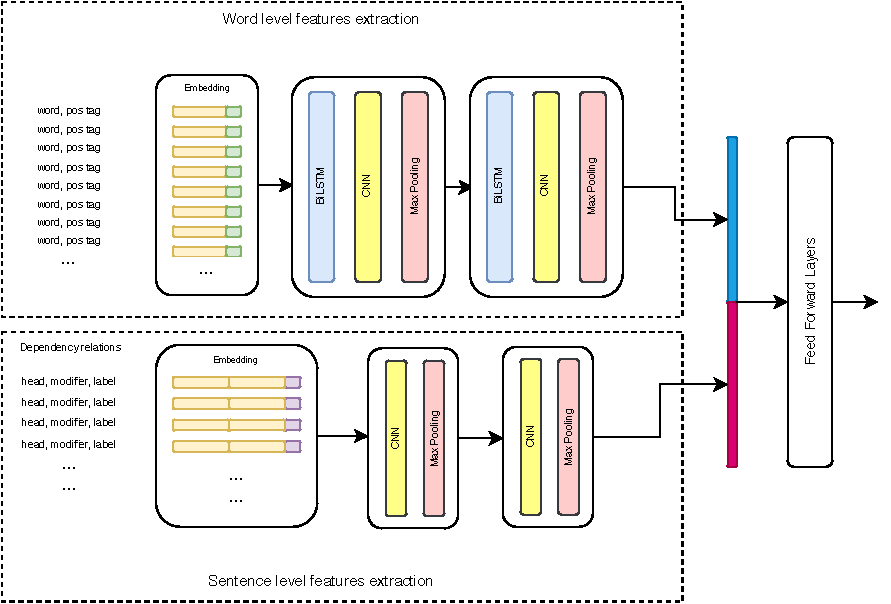
\includegraphics[width=0.75\textwidth]{model_arch.pdf}
	\caption{Final architecture}
	\label{fig:final_model}
\end{figure}

Our final architecture is informed by the findings of our previous experiments. It accepts five inputs: At the token-level, both  token
and part-of-speech tags (w/t punctuation) are used. Pre-trained GloVe embeddings are used for tokens, while embeddings for POS tags
are learned on-the-fly. The concatenation of both embeddings is passed through two "feature extraction units" that consist of a
BiLSTM (to target sequence/global information) and a 1D-Conv + MaxPool layer (to target local information). At sentence-level,
dependency information is encoded as the concatenation of the embeddings of the head word, modifier word and dependency label of each relation.
This is connected to two stripped-down "feature extraction units" without the BiLSTM layer, since dependency relations are
sequentially independent. Finally, the extracted representations of both token and sentence-level features are concatenated and
connected to a feed-forward layer and then a read-out layer.\\

The above architecture's separation of feature-extraction at token and sentential levels allows their information to be combined
at a higher level in the network. And we indeed see a marked improvement when this model is trained with dependency information.
The model achieved a best F1-score of $0.76$ during development.

\begin{table}[]
  \centering
  \resizebox{0.5\textwidth}{!}{%
  \begin{tabular}{@{}llcc@{}}
  \toprule
  \multicolumn{2}{c}{\multirow{2}{*}{\textbf{Hyperparameter}}} & \multicolumn{2}{c}{\textbf{Value}} \\ \cmidrule(l){3-4}
  \multicolumn{2}{c}{} & \textbf{Token-Level} & \textbf{Sentence-Level} \\ \midrule
  \multirow{3}{*}{\begin{tabular}[c]{@{}l@{}}Embeddings\\ Dim\end{tabular}} & Word & \multicolumn{2}{c}{300} \\
   & POS & \multicolumn{2}{c}{32} \\
   & Dep. Label & \multicolumn{2}{c}{32} \\ \midrule
  \multirow{4}{*}{\begin{tabular}[c]{@{}l@{}}Feature Extractor \\ Units\\ (Unit 1, Unit 2)\end{tabular}} & LSTM Units & 128, 64 & - \\
   & Conv. Filters & 128, 64 & 64, 32 \\
   & Conv. Kernel Size & \multicolumn{2}{c}{3, 3} \\
   & MaxPooling Pool Size & \multicolumn{2}{c}{2, 2} \\ \midrule
  \multicolumn{2}{l}{L2 Regularization $\beta$} & \multicolumn{2}{c}{0.001} \\
  \multicolumn{2}{l}{Feed-forward Units} & \multicolumn{2}{c}{24} \\ \bottomrule
  \end{tabular}%
  }
  \caption{Hyperparameters for the final model}
  \label{tab:final-hyperparameters}
\end{table}


\section{Results \& Discussion}
The final model achieved a positive-class F1-score of $0.6851$, ranking 47th out of 56 submissions for the first subtask. While the
model under-performed in a substantial departure from our expectations, we identified multiple factors that may have contributed to
it\footnote{Since the gold-standard data for the test set was not available at the time of publication, we based our statements on
our analysis of the training corpus and the prediction results of the test data.}. During training, we noticed that the number of
unique terms in the preprocessed corpus out-stripped the number of training samples (over 21K unique tokens in approx. 17K
sentences), over $75\%$ of which occurred only once. This inevitably results in a large pool over out-of-vocabulary words.
Pre-trained word embeddings trained on a relatively small corpus would be unable to model the vocabulary of the DEFT corpus completely,
particularly as the latter mostly comprises of domain-specific text. This could potentially be mitigated by restricting the
vocabulary based on term frequency count, but care must be taken not to restrict it too much as definitions, by definition, are
dependent on uniquely identifiable terms.\\

We also found several incongruities in the corpus where contradictions in annotations led to an ambiguous ground-truth. Consider the
following sentences from the training corpus: \emph{"Organisms are individual living entities."} and \emph{"Organelles are small
structures that exist within cells."} The first sentence was annotated with the positive class (contains a definition) even though the
latter was not. Another similar albeit more ambiguous example: \emph{"Recall from The Macroeconomic Perspective that if exports exceed imports, the economy is said to have a trade surplus."} and \emph{"If imports exceed exports, the economy is said to have a trade deficit."} Here, the second sentence is tagged as containing a definition even though the first isn't. While some of these
ambiguities can be attributed to how the training data for the binary classification task is generated from the larger sequence-annotated
corpus, there are many other counter-examples where the rationale behind the annotation is unclear. Such incongruities ultimately
make it more challenging for the model to attain a clear and optimal generalization.\\

And finally, on perhaps a more mundane note, real-world issues such as confusing instructions from the task organizers and
unreliable testing/submission infrastructure unfortunately also contributed to a less-than-optimal evaluation phase for our team.


\section{Conclusion}
We presented our system for definition extraction whose pre-BERT methods achieved an admittedly pre-historic F1-score of $0.6851$ in
Task 6: DeftEval, subtask 1. Future work could potentially include the customization of the architecture to incorporate ensemble training,
exploring the usage of more task-specific cues such as topical information, and perhaps even becoming one with the BERT side and using contextualized word embeddings.

\newpage
\bibliographystyle{coling}
\bibliography{semeval2020}



\end{document}
